\chapter{Primitive Types}

\section{Numbers}

% everything is a number, not always obvious, classes of numbers, the simples calls is integers
All values that we may want to work with in a computer are, one way or the other, \idx{numbers}{Number}. This fact may not always be obvious, but it will be quite a while before you encounter such examples. From public school and highschool, we know these classes of numbers:
\begin{itemize}
  \descitem{The \idx{natural numbers}{Numbers!Natural}} ($\mathbb{N}$) These are the non-negative numbers that can be written without a decimal point\footnote{There are two definitions of natural numbers. The other definition is that they are the positive numbers that can be written without a decimal point. That is to say, without zero. As this definition is generally less applicable in computers, we stick to the first definition.}.
  \descitem{The \idx{integers}{Numbers!Integer}} ($\mathbb{Z}$) These are all the natural numbers (according to the first definition) along with the negative versions of the natural numbers (according to the second definition). That definition juggling is to make sure that we don't have a negative zero.
  \descitem{The \idx{real numbers}{Numbers!Real}} ($\mathbb{R}$) These are all the numbers that can be placed on a line between $-\infty$ and $\infty$. We often refer to these as floating point numbers.
  \descitem{The \idx{rational numbers}{Numbers!Rational}} ($\mathbb{Q}$) These are then numbers that can be written as the fraction $m/n$ where $m \in \mathbb{Z}$ and $m \in \mathbb{N}$.
  \descitem{The \idx{irrational numbers}{Numbers!Irrational}} ($\mathbb{P}$) These are numbers that belong to $\mathbb{R}$ but not $\mathbb{Q}$. This is where $\pi$ and $e$ belong.
\end{itemize}
Computers typically works with other classes of numbers. In the following sections, we will explore the most commonly used ones. Common to these is that they are all \idx{represented in binary}{Representation!Binary} numbers. That is, using the \idx{base-2}{Base 2} digits. We are used to working with \idx{base-10}{Base 10} where numbers are digits between zero and nine. In base-2, the numbers are made up of digits between zero and one (i.e., \texttt{0} or \texttt{1}). Such a digit is called a \defi{bit}{Bit}, and a sequence of eight bits is referred to as a \defi{byte}{Byte}. The plural forms of the singular bit and byte is bits and bytes. Bits are, by the way, the \idx{SI unit}{SI unit} of information, in the same way as meter is the SI unit of distance. Accordingly, we measure \idx{information}{Information} in bits.

\section{Integers}

% how we know them (no decimal point), what we use them for (typically counts and variants thereof)
We recognize integers as numbers without a decimal point. We use them for counting, and variants thereof. A human may have two or three siblings. But if I were to tell you that I know someone who has 2.3 siblings then you would begin to question my faculties.

\subsection{Operations}

% basic operations
All general purpose languages support the four basic \idx{arithmetic operators}{Operation!Arithmetic} for addition, subtraction, multiplication and division of integers. The tree first of these will guarantee an integral result. For instance, if you add two integers, you will get an integer. The \textsl{size} of this integer may be affected though. But more on that in section \ref{primitives:int:representation}.

% that division thing
That rule, about the result of an operation resulting in an integral value does not hold for the \idx{division}{Operation!Division} operation though. Mathematically, the result \textsl{may} be integral, but generally speaking there is no guarantee, and more often than not it is simply not the case. Most programming languages supports two types of division; namely \idx{integer division}{Operation!Division!Integer} and \idx{floating-point division}{Operation!Division!Floating-point}. The result of a floating-point division is a floating-point number as introduced in section \ref{primitives:float}. The result of an integer division is an integer.

% remainder vs modulo
This operation is tightly coupled to both the \idx{remainder}{Remainder} and the \idx{modulo}{Modulo} operations. The difference between these is how they handle negative numbers.

% TODO: Figure of remainder vs modulo

\subsection{Representation}
\label{primitives:int:representation}

% intro: decimal (least significant digit to the right, 10 values for each digit, 10x difference between significance of neighboring digits), same for binary
We all know the \idx{decimal numeral system}{Decimal numeral system}. That is, the way we represent numbers using \idx{base-10}{Base-10} positioning of digits. In the west, we write the least significant digit to the right. There are ten potential values for each digit and a 10x order of magnitude between two successive digits. The same goes for \idx{binary}{Binary} (or \idx{base-2}{Base-2}). We write the least significant digit to the right, we have two potential values for each digit (zero and one), and the difference between two neighboring digits is a factor of two. Binary values are often \idx{prefixed}{Prefix!Number} by \say{0b}. Figure \ref{fig:prim:int:repr:base} illustrates how to interpret a binary number.

\begin{figure}[tbp]
  \begin{center}
  \begin{tikzpicture}[]
    \newcommand{\spacing}[0]{ 4mm }
    \tikzstyle{edge} = [thick ,draw=black]
    \tikzstyle{dedge} = [thick,->,>=stealth,draw=black]
    \tikzstyle{shared}=[
      anchor=center,
    ]
    \tikzstyle{structure}=[
      shared,
    ]
    \tikzstyle{digit}=[
      shared,
      text=teal,
      font=\ttfamily,
    ]
    \tikzstyle{label}=[
      font=\ttfamily,
    ]
    
    \node[matrix,row sep=\spacing,column sep=0mm,anchor=north,] () at (0,0) {
      % representations
      \node[digit] (bseven) {1};
      &
      &
      \node[digit] (bsix)   {0};
      &
      &
      \node[digit] (bfive)  {0};
      &
      &
      \node[digit] (bfour)  {1};
      &
      &
      \node[digit] (bthree) {1};
      &
      &
      \node[digit] (btwo)   {0};
      &
      &
      \node[digit] (bone)   {1};
      &
      &
      \node[digit] (bzero)  {1};
      &
      \node[label] (spacing spacing spacing) {\hspace{4mm}};
      &
      \node[digit] ()       {=};
      &
      \node[label] (spacing spacing spacing) {\hspace{4mm}};
      &
      \node[digit] (dtwo)   {1};
      &
      &
      \node[digit] (done)   {5};
      &
      &
      \node[digit] (dzero)  {5};
      \\
      
      % units
      \node[label] (bseven label) {$2^7$};
      &
      &
      \node[label] (bsix label)   {$2^6$};
      &
      &
      \node[label] (bfive label)  {$2^5$};
      &
      &
      \node[label] (bfour label)  {$2^4$};
      &
      &
      \node[label] (bthree label) {$2^3$};
      &
      &
      \node[label] (btwo label)   {$2^2$};
      &
      &
      \node[label] (bone label)   {$2^1$};
      &
      &
      \node[label] (bzero label)  {$2^0$};
      &
      &
      &
      &
      \node[label] (dtwo label)   {$10^2$};
      &
      &
      \node[label] (done label)   {$10^1$};
      &
      &
      \node[label] (dzero label)  {$10^0$};
      \\
      
      % values
      \node[label] (bseven value) {$128$};
      &
      \node[label] () {$+$};
      &
      \node[label] (bsix value)   {$0$};
      &
      \node[label] () {$+$};
      &
      \node[label] (bfive value)  {$0$};
      &
      \node[label] () {$+$};
      &
      \node[label] (bfour value)  {$16$};
      &
      \node[label] () {$+$};
      &
      \node[label] (bthree value) {$8$};
      &
      \node[label] () {$+$};
      &
      \node[label] (btwo value)   {$0$};
      &
      \node[label] () {$+$};
      &
      \node[label] (bone value)   {$2$};
      &
      \node[label] () {$+$};
      &
      \node[label] (bzero value)  {$1$};
      &
      &
      \node[label] () {$=$};
      &
      &
      \node[label] (dtwo value)   {$100$};
      &
      \node[label] () {$+$};
      &
      \node[label] (done value)   {$50$};
      &
      \node[label] () {$+$};
      &
      \node[label] (dzero value)  {$5$};
      \\
    };
    
    \draw[dedge] (bseven label)--(bseven);
    \draw[dedge] (bsix label)  --(bsix);
    \draw[dedge] (bfive label) --(bfive);
    \draw[dedge] (bfour label) --(bfour);
    \draw[dedge] (bthree label)--(bthree);
    \draw[dedge] (btwo label)  --(btwo);
    \draw[dedge] (bone label)  --(bone);
    \draw[dedge] (bzero label) --(bzero);
    \draw[dedge] (dtwo label)  --(dtwo);
    \draw[dedge] (done label)  --(done);
    \draw[dedge] (dzero label) --(dzero);
    
    \draw[edge] (bseven label)--(bseven value);
    \draw[edge] (bsix label)  --(bsix value);
    \draw[edge] (bfive label) --(bfive value);
    \draw[edge] (bfour label) --(bfour value);
    \draw[edge] (bthree label)--(bthree value);
    \draw[edge] (btwo label)  --(btwo value);
    \draw[edge] (bone label)  --(bone value);
    \draw[edge] (bzero label) --(bzero value);
    \draw[edge] (dtwo label)  --(dtwo value);
    \draw[edge] (done label)  --(done value);
    \draw[edge] (dzero label) --(dzero value);
    
    \draw[decorate,decoration={brace, amplitude=10pt, raise=5pt}] (bseven.north west) to node[black,midway,above=15pt] {binary (\textcolor{teal}{0b10011011})} (bzero.north east);
    \draw[decorate,decoration={brace, amplitude=10pt, raise=5pt}] (dtwo.north west) to node[black,midway,above=15pt] {decimal (\textcolor{teal}{155})} (dzero.north east);
  \end{tikzpicture}
\end{center}

  \caption{Representation of numbers in decimal and binary.}
  \label{fig:prim:int:repr:base}
\end{figure}

% hex
Often, you will also come across \idx{hexadecimal}{Hexadecimal} representation, which is still the same only \idx{base-16}{Base-16}. But here we run into a problem: While it is easy how to represent the ten lowest valued digits in a 16 digit system (i.e., 0 through 9), what do you the with the remaining six? How about eleven? Obviously, we could call it 11. But the consequence of that would be that we would either have to use two characters for each digit (e.g., 06 for 6), or rely on some other formatting trick (e.g., \{1,7,12,14,3\}) to be able to unambiguously decode a number. Both solutions are cumbersome and take up space. Instead, we usually say that eleven is \say{a}, twelve is \say{b} and so on. Then a digit is still a single character, and this allows us to write a number compactly. \idx{Hex values}{Value!Hex}, as these are called, are often prefixed by \say{0x}. An example of such a value is 0x04ff2b.

% binary example, and how to read it %TODO: Is this still relevant with the next paragraph?

% operations: essentially work like we are used to from decimal, ref to fig

\begin{figure}[tbp]
  % 2+4+16 = 22
% 1+4+16+32 = 53
% 22 + 53 = 75
% 1+2+8+64 = 75

\begin{center}
  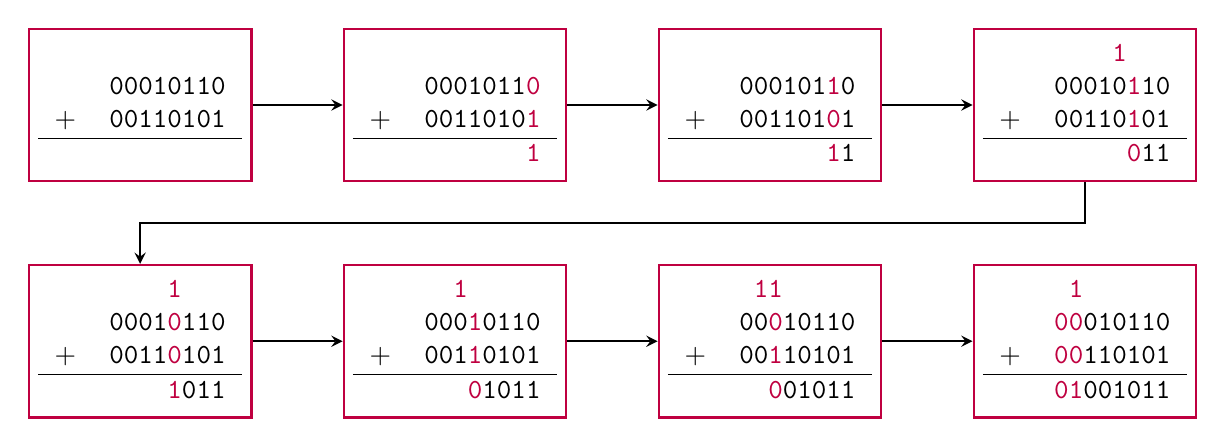
\begin{tikzpicture}[remember picture]
    \newcommand{\xStep}[0]{4cm}
    \newcommand{\yStep}[0]{3cm}
    \newcommand{\highl}[1]{\textcolor{purple}{#1}}
    \newcommand{\charspace}[0]{\textcolor{white}{0}}
    
    \tikzstyle{dedge} = [thick,->,>=stealth,draw=black]
    
    \tikzstyle{node}=[
      rectangle,
      draw=purple,
      anchor=center,
      thick,
      minimum size=1,
    ]
    
    \node[node] (n1) at (0*\xStep,0*\yStep) {
      \begin{tabular}{lr}
          & \texttt{} \\
          & \texttt{00010110} \\
        + & \texttt{00110101} \\
        \hline
          & \texttt{} \\
      \end{tabular}
    };
    
    \node[node] (n2) at (1*\xStep,0*\yStep) {
      \begin{tabular}{lr}
          & \texttt{} \\
          & \texttt{0001011\highl{0}} \\
        + & \texttt{0011010\highl{1}} \\
        \hline
          & \texttt{\highl{1}} \\
      \end{tabular}
    };
    
    \node[node] (n3) at (2*\xStep,0*\yStep) {
      \begin{tabular}{lr}
          & \texttt{} \\
          & \texttt{000101\highl{1}0} \\
        + & \texttt{001101\highl{0}1} \\
        \hline
          & \texttt{\highl{1}1} \\
      \end{tabular}
    };
    
    \node[node] (n4) at (3*\xStep,0*\yStep) {
      \begin{tabular}{lr}
          & \texttt{\highl{1}\charspace\charspace\charspace} \\
          & \texttt{00010\highl{1}10} \\
        + & \texttt{00110\highl{1}01} \\
        \hline
          & \texttt{\highl{0}11} \\
      \end{tabular}
    };
    
    \node[node] (n5) at (0*\xStep,-1*\yStep) {
      \begin{tabular}{lr}
          & \texttt{\highl{1}\charspace\charspace\charspace} \\
          & \texttt{0001\highl{0}110} \\
        + & \texttt{0011\highl{0}101} \\
        \hline
          & \texttt{\highl{1}011} \\
      \end{tabular}
    };
    
    \node[node] (n6) at (1*\xStep,-1*\yStep) {
      \begin{tabular}{lr}
          & \texttt{\highl{1}\charspace\charspace\charspace\charspace\charspace} \\
          & \texttt{000\highl{1}0110} \\
        + & \texttt{001\highl{1}0101} \\
        \hline
          & \texttt{\highl{0}1011} \\
      \end{tabular}
    };
    
    \node[node] (n7) at (2*\xStep,-1*\yStep) {
      \begin{tabular}{lr}
          & \texttt{\highl{1}\highl{1}\charspace\charspace\charspace\charspace\charspace} \\
          & \texttt{00\highl{0}10110} \\
        + & \texttt{00\highl{1}10101} \\
        \hline
          & \texttt{\highl{0}01011} \\
      \end{tabular}
    };
    
    \node[node] (n8) at (3*\xStep,-1*\yStep) {
      \begin{tabular}{lr}
          & \texttt{\highl{1}\charspace\charspace\charspace\charspace\charspace\charspace} \\
          & \texttt{\highl{00}010110} \\
        + & \texttt{\highl{00}110101} \\
        \hline
          & \texttt{\highl{01}001011} \\
      \end{tabular}
    };
    
    \draw[dedge] (n1)--(n2);
    \draw[dedge] (n2)--(n3);
    \draw[dedge] (n3)--(n4);
    \draw[dedge] (n4)|-(1.5*\xStep,-0.5*\yStep)-|(n5);
    \draw[dedge] (n5)--(n6);
    \draw[dedge] (n6)--(n7);
    \draw[dedge] (n7)--(n8);
  \end{tikzpicture}
\end{center}

  \caption{Addition of two 8-bit binary numbers.}
  \label{fig:prim:int:binary:add}
\end{figure}

% signedness: two's compliment

\csharpsubsection{\csharp}

\begin{syntaxfloat}
  \begin{syntax}{expr}
  \SyntaxWestSplit{MainWest}
  \SyntaxEastSplit{MainEast}
  
  \node[nonterminal] (ruleIa)  at \SyntaxDistribute{MainWest}{MainEast}{1}{3} {expr};
  \node[terminal]    (ruleIb)  at \SyntaxDistribute{MainWest}{MainEast}{2}{3} {+};
  \node[nonterminal] (ruleIc)  at \SyntaxDistribute{MainWest}{MainEast}{3}{3} {expr};
  \node[nonterminal] (ruleIIa) at \SyntaxDistributeLine{MainWest}{MainEast}{1}{3}{1} {expr};
  \node[terminal]    (ruleIIb) at \SyntaxDistributeLine{MainWest}{MainEast}{2}{3}{1} {-};
  \node[nonterminal] (ruleIIc) at \SyntaxDistributeLine{MainWest}{MainEast}{3}{3}{1} {expr};
  \node[nonterminal] (ruleIIIa) at \SyntaxDistributeLine{MainWest}{MainEast}{1}{3}{2} {expr};
  \node[terminal]    (ruleIIIb) at \SyntaxDistributeLine{MainWest}{MainEast}{2}{3}{2} {*};
  \node[nonterminal] (ruleIIIc) at \SyntaxDistributeLine{MainWest}{MainEast}{3}{3}{2} {expr};
  \node[nonterminal] (ruleIVa) at \SyntaxDistributeLine{MainWest}{MainEast}{1}{3}{3} {expr};
  \node[terminal]    (ruleIVb) at \SyntaxDistributeLine{MainWest}{MainEast}{2}{3}{3} {/};
  \node[nonterminal] (ruleIVc) at \SyntaxDistributeLine{MainWest}{MainEast}{3}{3}{3} {expr};
  \node[nonterminal] (ruleVa) at \SyntaxDistributeLine{MainWest}{MainEast}{1}{3}{4} {expr};
  \node[terminal]    (ruleVb) at \SyntaxDistributeLine{MainWest}{MainEast}{2}{3}{4} {\%};
  \node[nonterminal] (ruleVc) at \SyntaxDistributeLine{MainWest}{MainEast}{3}{3}{4} {expr};
  
  \draw[path] (begin)--(ruleIa)--(ruleIb)--(ruleIc)--(end);
  \draw[path] (begin) to[-|-] (ruleIIa)--(ruleIIb)--(ruleIIc) to[-|-] (end);
  \draw[path] (begin) to[-|-] (ruleIIIa)--(ruleIIIb)--(ruleIIIc) to[-|-] (end);
  \draw[path] (begin) to[-|-] (ruleIVa)--(ruleIVb)--(ruleIVc) to[-|-] (end);
  \draw[path] (begin) to[-|-] (ruleVa)--(ruleVb)--(ruleVc) to[-|-] (end);
\end{syntax}

  \caption{Expressions of arithmetic operators}
  \label{syntax:prim:arithmetic:ops}
\end{syntaxfloat}

% integer types available

\begin{figure}[tbp]
  \begin{center}
  \begin{tabular}{rccl}
    \emph{Size} & \emph{Unsigned Type} & \emph{Signed Type} & \emph{Comment} \\
     8 bits & \typename{byte} & \typename{sbyte} & \\
    16 bits & \typename{ushort} & \typename{short} & \\
    32 bits & \typename{uint} & \typename{int} & \\
    64 bits & \typename{ulong} & \typename{long} & \\
    1 word & \typename{nuint} & \typename{nint} & Do not use\\
  \end{tabular}
\end{center}

  \caption{Integer types available in \csharp.}
  \label{fig:prim:int:csharp:types}
\end{figure}

% what is the result of int32+int32? what is an overflow?

\elixirsubsection{Elixir}

% arbitrary sizes: pros
In Elixir, there is only one integer type and that has an \idx{arbitrary size}{Arbitrary size}. As long as an integral value fits in memory, an Elixir integer can hold it. The value is not in having integers that each take up 90\% of your \idx{primary memory}{Memory!Primary}. It is very rare that we have a need for integers beyond 128 bits or even 64 bits. But when we work with \idx{fixed size}{Fixed size} integers, we always have to be aware of that hard limit. In Elixir, we don't have to: If we somehow end up with a number needing 7000 bits, then that is what gets allocated. We don't have to worry.

% and cons, why the tradeoff was resolved in this way
Elixir code, still runs on the same hardware though. This hardware does not have instructions capable of operating on 7000 bit integers. So, instead of an integer operation being a single \idx{instruction}{Instruction}, it is an \idx{algorithm}{Algorithm} in itself. This is significantly slower. Elixir is designed for network intensive tasks, and these are even slower. So, for the tasks where one would choose Elixir, it basically doesn't matter. And that is why the designers of that language has made that choice.

\section{Floating Point Numbers}
\label{primitives:float}

\subsection{Operations}
\subsection{Representation}
\csharpsubsection{\csharp}
\elixirsubsection{Elixir}

\section{Truth Values}
\label{primitives:bools}

% what do they represent

\subsection{Operations on Nontruthy Values}

Any valid comparison between two nontruthy values will yield a truthy value. For instance, if we ask \quoted{is 42 equal to 56?} then the resulting value is \valuename{false} but if we ask \quoted{is 1 less than or equal to 2?} then the resulting value is \valuename{true}. The full set of comparison operators are listed in figure \ref{fig:prim:bool:comparison}. This is one of the primary ways of creating boolean values.

\begin{figure}[tbp]
  \begin{center}
  \begin{tabular}{cl}
    $a$ \texttt{==} $b$ & True if $a$ is the same as $b$ \\
    $a$ \texttt{!=} $b$ & True if $a$ is different from $b$ \\
    $a$ \texttt{<} $b$ & True if $a$ is less than $b$ \\
    $a$ \texttt{<=} $b$ & True if $a$ is less than or equal to $b$ \\
    $a$ \texttt{>} $b$ & True if $a$ is greater than $b$ \\
    $a$ \texttt{>=} $b$ & True if $a$ is greater than or equal to $b$ \\
  \end{tabular}
\end{center}

  \caption{Comparison operators.}
  \label{fig:prim:bool:comparison}
\end{figure}

\subsection{Operations on Truth Values}

\begin{figure}[tbp]
  \begin{center}
  \begin{tabular}{cccccc}
    $a$ & $b$ & $a \wedge b$ & $a \vee b$ & $a \oplus b$ & $\neg a$\\
    0 & 0 & 0 & 0 & 0 & 1 \\
    0 & 1 & 0 & 1 & 1 & \\
    1 & 0 & 0 & 1 & 1 & 0 \\
    1 & 1 & 1 & 1 & 0 & \\
  \end{tabular}
\end{center}

  \caption{Truth table for the boolean operations.}
  \label{fig:prim:bool:and}
\end{figure}

% TODO: De Morgan's law

\subsection{Representation}

% technically a bit, but typically (mostly unless in array form) a byte or word

\csharpsubsection{\csharp}

\begin{syntaxfloat}
  \begin{syntax}{expr}
  \SyntaxWestSplit{MainWest}
  \SyntaxEastSplit{MainEast}
  
  \node[sequence] () at ([yshift=0*\syntaxruledist]$(begin)!0.5!(end)$) {
    \node[nonterminal] (ruleIa) {expr};
    &
    \node[terminal]    (ruleIb) {\&\&};
    &
    \node[nonterminal] (ruleIc) {expr};
    \\
  };
  
  \node[sequence] () at ([yshift=-1*\syntaxruledist]$(begin)!0.5!(end)$) {
    \node[nonterminal] (ruleIIa) {expr};
    &
    \node[terminal]    (ruleIIb) {||};
    &
    \node[nonterminal] (ruleIIc) {expr};
    \\
  };
  
  \node[sequence] () at ([yshift=-2*\syntaxruledist]$(begin)!0.5!(end)$) {
    \node[nonterminal] (ruleIIIa) {expr};
    &
    \node[terminal]    (ruleIIIb) {\^{}};
    &
    \node[nonterminal] (ruleIIIc) {expr};
    \\
  };
  
  \node[sequence] () at ([yshift=-3*\syntaxruledist]$(begin)!0.5!(end)$) {
    \node[terminal]    (ruleIVa) {!};
    &
    \node[nonterminal] (ruleIVb) {expr};
    \\
  };
  
  \draw[path] (begin)--(ruleIa)--(ruleIb)--(ruleIc)--(end);
  \draw[path] (begin) to[-|-] ([xshift=4cm,yshift=-1*\syntaxruledist]begin.east)--(ruleIIa)--(ruleIIb)--(ruleIIc)--([xshift=-4cm,yshift=-1*\syntaxruledist]end.west) to[-|-] (end);
  \draw[path] (begin) to[-|-] ([xshift=4cm,yshift=-2*\syntaxruledist]begin.east)--(ruleIIIa)--(ruleIIIb)--(ruleIIIc)--([xshift=-4cm,yshift=-2*\syntaxruledist]end.west) to[-|-] (end);
  \draw[path] (begin) to[-|-] ([xshift=4cm,yshift=-3*\syntaxruledist]begin.east)--(ruleIVa)--(ruleIVb)--([xshift=-4cm,yshift=-3*\syntaxruledist]end.west) to[-|-] (end);
\end{syntax}

  \caption{Expressions of boolean operators}
  \label{syntax:prim:bool:ops}
\end{syntaxfloat}

\elixirsubsection{Elixir}

\csubsection{C}

% low-level language
\idx{C}{Language!C} is a simple \idx{low-level language}{Language!Low-level}. That means that it mirrors the fundamental properties of the underlying harware and adds some highly convenient abstractions. These abstractions are chosen is such a way that they essentially can be delivered without a performance overhead.

% consequence: a boolean is a register
\idxx{Machine code} does not have a boolean type. Instead \idx{register}{Register} values that are represented using all zeroes in binary are \textsl{false} and every other value is \textsl{true}. That means -- in terms of integers -- that zero is \textsl{false} and non-zero is \textsl{true}. % TODO: Explain the !!42 == 1 situation, word for reference/strong true values, implicit konvertering til bool i condition af en if

% consequence: a bool is an integer and can thus be used in an integer expression
A consequence of this is that C doesn't have a notion of a \idx{boolean}{Boolean}. Instead, integers are used: A boolean is an interpretation of an integer, and can thus be used in an integer expression. Typically, this will make absolutely no difference. Proponents of \csharp\ will point out that booleans and integers are fundamentally different notions and should thus be treated differently. Proponents of C will point out that this allows them to write code such as this:

% TODO: Example

% explanation: why is this clever (no branches gives execution speed, and it is still readable)

\section{Local Variables}
\csharpsubsection{\csharp}

\begin{syntaxfloat}
  \begin{syntax}[[xshift=22mm]concept.west]{type}
  \SyntaxWestSplit{MainWest}
  \SyntaxEastSplit{MainEast}
  
  \node[terminal] (ruleIa) at ($(begin)!0.5!(end)$) {name};
  
  \draw[path] (begin)--(ruleIa)--(end);
\end{syntax}
\begin{syntax}[[xshift=22mm]concept.west]{local-var}
  \SyntaxWestSplit{MainWest}
  \SyntaxEastSplit{MainEast}
  
  \node[sequence,anchor=north] () at ([yshift=\syntaxrulenodeheight-0.8pt*3]$(begin.east)!0.5!(end.west)$) {
    \node[nonterminal] (ruleIa) {type};
    &
    \node[terminal]    (ruleIb) {name};
    &
    \node[terminal]    (ruleIc) {=};
    &
    \node[nonterminal] (ruleId) {expr};
    &
    \node[terminal]    (ruleIe) {;};
    \\
    \node[nonterminal] (ruleIIa) {type};
    &
    \node[terminal]    (ruleIIb) {name};
    &
    &
    &
    \node[terminal]    (ruleIIc) {;};
    \\
  };
  
  \draw[path] (begin)--(ruleIa)--(ruleIb)--(ruleIc)--(ruleId)--(ruleIe)--(end);
  \draw[path] (begin) to[-|-] ([xshift=2cm,yshift=-1*(\syntaxruledist+0.8pt*3)]begin.east)--(ruleIIa)--(ruleIIb)--(ruleIIc)--([xshift=-2cm,yshift=-1*(\syntaxruledist+0.8pt*3)]end.west) to[-|-] (end);
\end{syntax}
\begin{syntax}[[xshift=22mm]concept.west]{stmt}
  \SyntaxWestSplit{MainWest}
  \SyntaxEastSplit{MainEast}
  
  \node[nonterminal] (ruleIa) at ($(begin)!0.5!(end)$) {local-var};
  
  \draw[path] (begin)--(ruleIa)--(end);
\end{syntax}


  \caption{Local variables.}
  \label{syntax:prim:vars:locals}
\end{syntaxfloat}

\elixirsubsection{Elixir}

\section{Parsing}
\subsection{Operator Precedence}

% parentheses

\subsection{Operator Associativity}

\csharpsubsection{\csharp}

\begin{syntaxfloat}
  \begin{syntax}{expr}
  \SyntaxWestSplit{MainWest}
  \SyntaxEastSplit{MainEast}
  
  \node[sequence] () at ([yshift=0*\syntaxruledist]$(begin)!0.5!(end)$) {
    \node[terminal]    (ruleIa) {(};
    &
    \node[nonterminal] (ruleIb) {expr};
    &
    \node[terminal]    (ruleIc) {)};
    \\
  };
  
  \draw[path] (begin)--(ruleIa)--(ruleIb)--(ruleIc)--(end);
\end{syntax}

  \caption{Expressions of parentheses}
  \label{syntax:prim:pars}
\end{syntaxfloat}

\exercises{primitives}{Primitive Types}

